\documentclass[12pt]{article}

\usepackage[margin=1in]{geometry}
\usepackage[T1]{fontenc}
\usepackage[utf8]{inputenc}
\usepackage{kotex}
\usepackage{graphicx}
\usepackage{underscore}
\usepackage[sort]{natbib}
\usepackage{booktabs}
\usepackage{amsmath}
\usepackage{subcaption}
\usepackage[hidelinks]{hyperref}
\usepackage{setspace}
\doublespacing

\graphicspath{{../output/figures/}}

\title{코리아 디스카운트: 기업지배구조 결함, 구조적 개혁,\\그리고 자율적 개입의 한계}
\author{Daniel Jung}
\date{2026년 5월 8일}

\begin{document}
\maketitle

\begin{abstract}
한국 주식시장은 30년 넘게 선진국·신흥국 시장보다 구조적으로 낮은 밸류에이션을 유지해왔다. 이 보고서는 코리아 디스카운트를 다룬 기존 연구를 정리하고, 20년 치 월별 지수 P/B 패널 데이터에서 얻은 실증 결과를 제시한다. 선행 문헌은 크게 세 가지 설명---재벌 소유구조와 터널링, 소수 주주 보호 미비, 성장 기초 여건 정체---으로 모아지지만, 어느 요인이 더 중요한지에 대해서는 의견이 갈린다. 횡단면 회귀분석 (cross-sectional regression)에서는 성장을 통제하면 공식 지배구조 점수가 유의하지 않고 \citep{yang2025korea}, 자연 실험 (natural experiment)들은 소유구조 기반 자기거래가 직접적인 가치 파괴임을 보여준다 \citep{black2015governance}. 일본의 지배구조 개혁 세 차례를 벤치마크로 삼은 스택형 사건 연구 (stacked event study) 결과, 자율적인 2014년 스튜어드십 코드와 2015년 기업지배구조 코드 이후에는 지속적인 재평가가 나타나지 않았다. 반면 2023년 TSE P/B 개혁 요청 이후 24개월 동안 KOSPI--TOPIX 누적 스프레드는 $-6.48$ P/B 포인트에 달했고, 2025년 구속력 있는 의무화 이후 격차는 더 벌어졌다. 아직 자율적 성격을 유지하는 한국의 2024년 기업가치 제고 프로그램 이후에는 밸류에이션 개선이 나타나지 않았다: MSCI EM 아시아는 세 이정표 모두에서 $\tau=12$ 기준 KOSPI를 각각 $+2.18$, $+1.80$, $+2.12$ P/B 포인트 상회했다. 또한 지정학적 리스크 반증 (falsification) 분석은 급성 지정학적 충격이 할인의 원인이라는 설명을 기각한다 ($t=-0.84$, $p=0.40$). 전체 증거는 연성 지배구조 규범보다 집행 신뢰성을 갖춘 개혁을 지지한다.
\end{abstract}

\section{서론}
\label{sec:intro}

``코리아 디스카운트''---글로벌 시장 대비 한국 주식의 지속적 저평가---는 국제 금융에서 가장 오래된 수수께끼 중 하나다. 2004--2024년 동안 KOSPI P/B는 TOPIX보다 평균 $0.177\times$ 낮고 ($t=-3.23$), MSCI EM보다 $0.601\times$ 낮다 ($t=-10.31$). 두 격차 모두 Newey-West HAC 표준오차 기준으로 통계적으로 유의하다. 이 할인은 적어도 30년째 계속되고 있으며, 일본의 2025년 지배구조 개혁 의무화 이후 더 벌어졌고, 한국의 2024년 자율적 기업가치 제고 프로그램으로도 줄지 않았다.

이 보고서의 기여는 두 가지다. 첫째, 한국어 학술지 게재 11편을 포함해 21편의 연구를 할인에 대한 경쟁적 설명---지배구조와 터널링, 성장 기초 여건, 기관투자자 스튜어드십---별로 정리한다. 둘째, 일본의 단계적 지배구조 개혁을 정책 벤치마크로 써서 KOSPI, TOPIX, S\&P~500, MSCI~EM을 아우르는 20년 치 월별 패널 데이터에서 새로운 실증 결과를 내놓는다. 핵심 실증 패턴은 이렇다: 일본의 2014--2015년 연성 규범 같은 자율적 지배구조 코드 이후에는 꾸준한 밸류에이션 개선이 뒤따르지 않았다. 반면 준수 현황의 공개적 공시와 암묵적 시장 강등 압박으로 뒷받침된 거래소 집행---일본 2023년 TSE P/B 개혁 요청이 그 사례---이후에는 스프레드 확대가 관찰됐다.

\section{할인의 정의와 측정}
\label{sec:measurement}

코리아 디스카운트는 동종 시장 대비 낮은 P/B 및 P/E로 나타나는 한국 주식의 고질적인 저평가를 의미한다. 가장 철저한 국제 증거는 1990년부터 2023년까지 48개국 데이터를 통해, 기업 규모·수익성·성장성·1인당 GDP·금융시장 발전도·지정학적 리스크를 모두 통제한 뒤에도 한국 기업의 P/B·P/E 배수가 지속적으로 낮음을 보여준다 \citep{kim2026korean}. 이 결과는 1990년대, 2000년대, 2010년대 이후 모든 세부 기간에 걸쳐 유지된다. 결국 할인은 단순한 경기 탓이 아니라 구조적인 것이다.

할인이 리스크를 반영하는 것인지, 아니면 가격 오류인지에 대해서는 논란이 있다. 장부가 대비 시장가 (book-to-market, BTM) 비율이 1을 넘는 한국 기업들은 BTM이 낮은 기업들보다 일관되게 높은 성과를 냈다. 게다가 높은 BTM은 긍정적 극단 수익의 확률이 높고 부정적 극단 수익의 확률이 낮은 것과 연관된다---이건 리스크 보상이 아니라 가격 오류라는 뜻이다 \citep{jung2022korea}. 그중에서도 지배구조 요인이 가장 강력한 횡단면 예측 변수 (cross-sectional predictor)였다.

그림~\ref{fig:pb_comparison}은 20년간의 P/B 궤적을 보여준다. 표~\ref{tab:summary_stats}은 핵심 통계를 정리한다. KOSPI--TOPIX 스프레드 평균은 $-0.177\times$ (NW SE $= 0.055$, $t=-3.23$, 95\% CI: $[-0.284, -0.069]$), KOSPI--MSCI EM 스프레드는 $-0.601\times$ (NW SE $= 0.058$, $t=-10.31$, 95\% CI: $[-0.716, -0.486]$)다. 세부 기간을 나눠보면 구조적 악화가 뚜렷하다: KOSPI--TOPIX 격차는 2004--2013년 P/B 0.05 포인트에서 2023--2024년 0.43 포인트로 벌어졌다. 다만 섹터 구성은 주의해서 봐야 한다. KOSPI는 경기순환형 하드웨어 제조업에 집중되어 있어(삼성전자와 SK하이닉스만이 지수 가중치의 약 30\%를 차지), TOPIX와 S\&P~500이 소프트웨어·서비스·소비재 같이 구조적으로 높은 P/B 배수를 기록하는 섹터의 비중이 더 크다. \citet{kim2026korean}은 48개국 기업 수준 특성을 통제한 후에도 할인이 유지됨을 보여주지만, 여기서 보고된 지수 수준 스프레드는 섹터 가중치를 조정하지 않는다.

\begin{figure}[htbp]
    \centering
    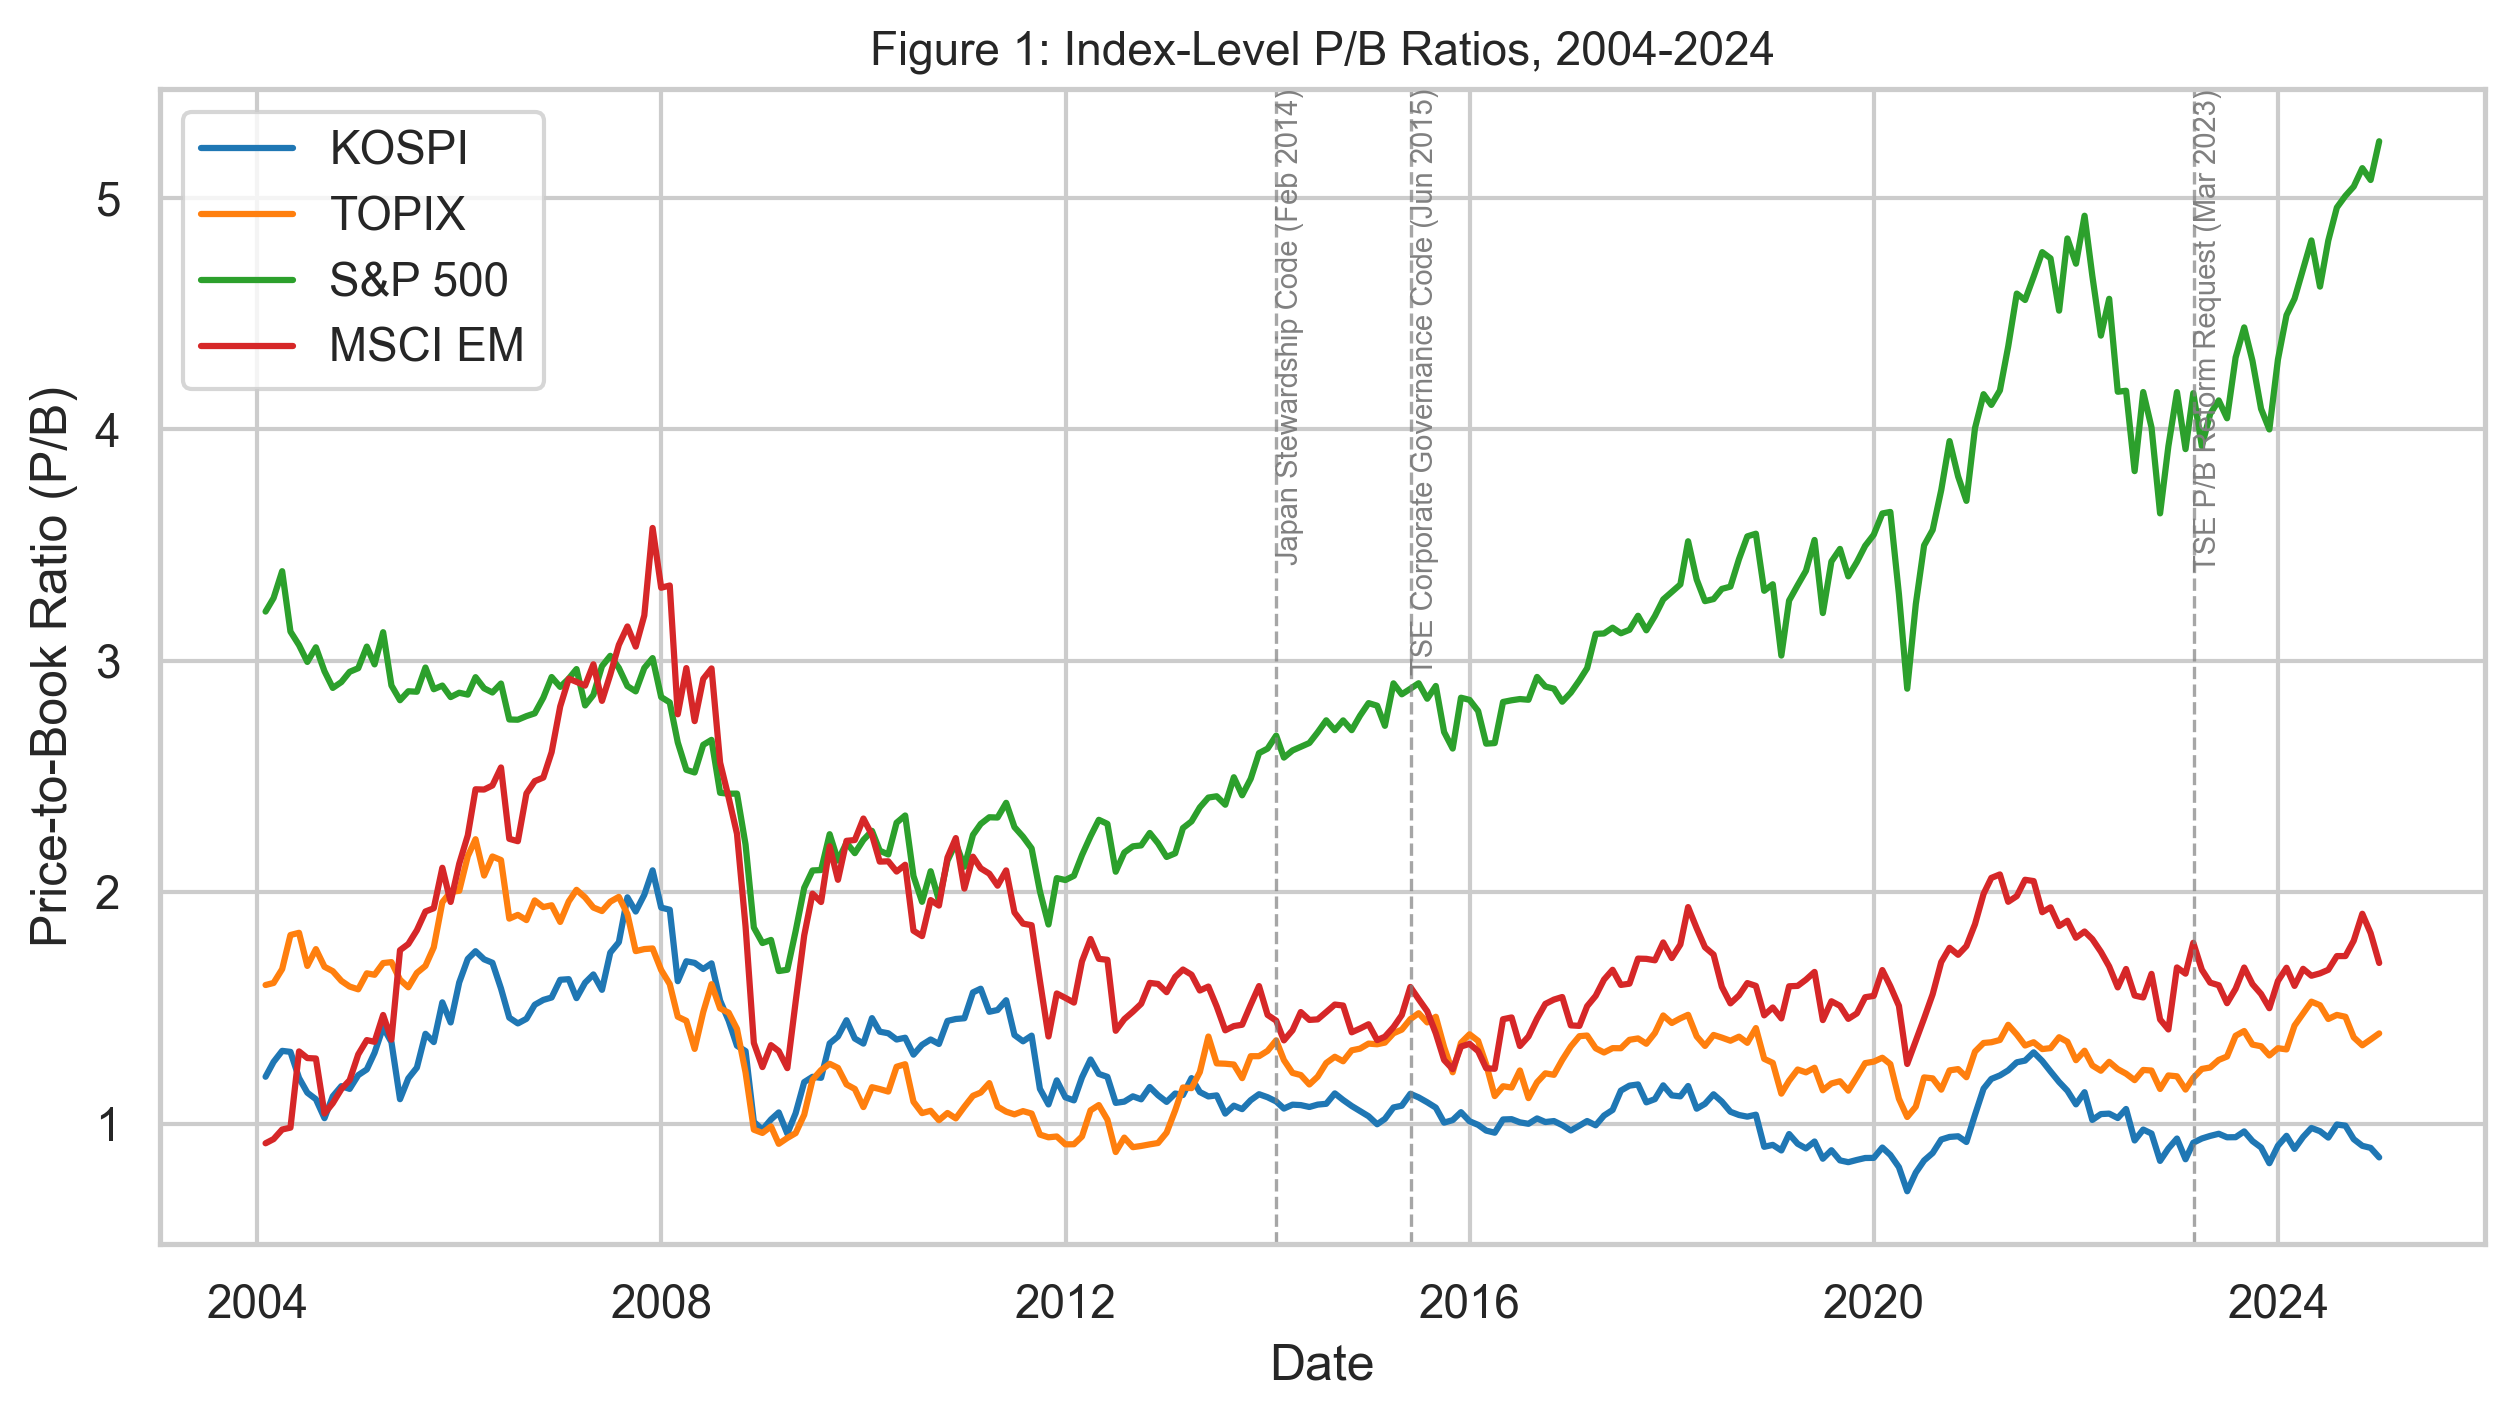
\includegraphics[width=0.95\textwidth]{figure1_pb_comparison.png}
    \caption{월별 P/B 비율, 2004년 1월--2024년 12월. 수직선은 일본의 지배구조 개혁 이정표를 표시한다.}
    \label{fig:pb_comparison}
\end{figure}

\begin{table}
\caption{Summary statistics of index-level P/B ratios by country and sub-period.}
\label{tab:summary_stats}
\begin{tabular}{llrrrrr}
\toprule
 & Period & mean & median & std & min & max \\
country &  &  &  &  &  &  \\
\midrule
KOSPI & Full (2004--2024) & 1.18 & 1.10 & 0.26 & 0.71 & 2.09 \\
MSCI\_EM & Full (2004--2024) & 1.78 & 1.65 & 0.47 & 0.91 & 3.58 \\
SP500 & Full (2004--2024) & 3.08 & 2.89 & 0.81 & 1.66 & 5.25 \\
TOPIX & Full (2004--2024) & 1.35 & 1.31 & 0.28 & 0.88 & 2.23 \\
KOSPI & Pre-reform (2004--2013) & 1.36 & 1.34 & 0.25 & 0.96 & 2.09 \\
MSCI\_EM & Pre-reform (2004--2013) & 1.97 & 1.91 & 0.60 & 0.91 & 3.58 \\
SP500 & Pre-reform (2004--2013) & 2.51 & 2.42 & 0.40 & 1.66 & 3.39 \\
TOPIX & Pre-reform (2004--2013) & 1.41 & 1.29 & 0.39 & 0.88 & 2.23 \\
KOSPI & Reform era (2014--2022) & 1.02 & 1.03 & 0.12 & 0.71 & 1.31 \\
MSCI\_EM & Reform era (2014--2022) & 1.59 & 1.55 & 0.20 & 1.24 & 2.08 \\
SP500 & Reform era (2014--2022) & 3.39 & 3.28 & 0.63 & 2.58 & 4.92 \\
TOPIX & Reform era (2014--2022) & 1.29 & 1.28 & 0.10 & 1.03 & 1.48 \\
KOSPI & Post-TSE (2023--2024) & 0.93 & 0.94 & 0.04 & 0.83 & 1.00 \\
MSCI\_EM & Post-TSE (2023--2024) & 1.66 & 1.66 & 0.10 & 1.50 & 1.91 \\
SP500 & Post-TSE (2023--2024) & 4.51 & 4.47 & 0.43 & 3.91 & 5.25 \\
TOPIX & Post-TSE (2023--2024) & 1.36 & 1.35 & 0.10 & 1.15 & 1.53 \\
\bottomrule
\end{tabular}
\end{table}


\section{지배구조 채널: 재벌, 터널링, 자기거래}
\label{sec:governance}

\subsection{재벌 소유구조와 터널링}

코리아 디스카운트의 구조적 뿌리는 한국 경제를 지배하는 가족 지배 대기업 집단, 즉 재벌에 있다. 재벌 형성 과정을 추적한 연구에 따르면, 지배 가족들은 피라미드 구조 속에서 수익성이 낮은 기업을 인수하기 위해 ``중심 기업''을 쓴다. 이 중심 기업들은 할인된 가격에 거래됐는데, 이건 가치 파괴적 인수를 예상한 주주들의 반응이다 \citep{almeida2011chaebol}.

터널링의 경제적 규모는 크다. 재벌 계열사가 인수를 진행하면 해당 기업 주가는 평균적으로 떨어지는 반면, 지배 주주는 다른 그룹 계열사로의 가치 이전을 통해 이익을 챙긴다 \citep{bae2002tunneling}. 기업집단 계열사들은 또 체계적으로 더 많은 기부를 하는데, 이 기부는 가족이 낮은 현금흐름권을 보유한 공개 계열사에서 높은 지분을 가진 비공개 계열사로 자원을 빼돌리는 수단이다 \citep{kim2019tunneling}.

터널링 유인은 한국의 세제 때문에 더 강해진다. 한국은 대기업 지배주주의 상속세율이 최고 60\%에 달하는 OECD 최고 수준이며, 배당소득도 최고 45\%의 한계세율로 과세된다. 부가 가치가 그룹 지분에 집중된 지배 가족에게는 주가 상승이 곧 승계 세부담의 증가를 의미한다. 이는 낮은 배당, 계열사 간 가치 이전, 주가 억제를 통해 밸류에이션을 의도적으로 낮추는 합리적 유인을 만든다. 이런 세제 구조 아래에서 터널링은 단순한 기회주의가 아니라 개인적으로 최적인 선택이 된다: 공개 계열사의 밸류에이션을 낮게 유지함으로써 지배 주주는 세대 간 승계의 재정적 비용과 적대적 인수자에게 지배권을 잃을 위험을 동시에 줄일 수 있다.

\subsection{자연 실험 (Natural Experiment) 증거}

대형 기업에 더 엄격한 이사회 요건을 요구한 한국의 1999년 개혁을 활용한 연구는 강력한 인과 증거를 제공한다. 사건 연구 (event study) 결과, 터널링 유인을 가진 지배주주가 있는 대형 기업들이 강한 양(+)의 비정상 수익률 (abnormal return)을 기록했다. 패널 회귀분석 (panel regression)도 같은 결론을 뒷받침한다: 지배구조 개선은 관계사 거래가 기업 가치를 갉아먹는 효과를 줄였고, 기업 수익성이 산업 흐름을 더 잘 따라가게 했다. 이건 터널링이 줄었다는 신호다 \citep{black2015governance}.

집중된 소유구조는 더 넓은 지배구조 환경도 왜곡한다. 재벌 계열사들 사이에서는 주주권 보호만이 배당 성향에 대한 설명력을 유지했고, 이사회 효과성·감사 역량·공시 투명성은 소유구조를 통제하면 독립적 영향력을 잃었다 \citep{njoku2026governance}.

재벌의 또 다른 특징은 지정 지주회사다. 법적으로 지정된 지주회사는 운영 회사 및 기초 가치 대비 상당한 P/B 할인으로 거래된다---일본과 미국에서는 나타나지 않는 한국 특유의 현상이다 \citep{park2019holding}. 교차 주식 보유 의결권 제한은 지주회사를 경영권 쟁탈에 노출시켜 재평가를 유도할 수 있다 \citep{park2025cross}. 다만 이는 근본적인 지배구조 개선이라기보다 방어적 전술에 가깝다. 초다수결 경영권 방어 조항을 약화시킨 법원 판결 분석에서는 해당 조항을 보유한 기업들이 더 높은 성과를 냈는데, 이건 남용 없이 쓰일 때 가치를 높이는 기능을 한다는 뜻이다 \citep{kim2022supermajority}.

\section{성장 대 지배구조 논쟁}
\label{sec:growth}

제~\ref{sec:governance}절의 터널링·자기거래 증거는 지배구조를 할인의 주된 원인으로 강하게 지지한다. 그러나 이에 반하는 것처럼 보이는 횡단면 (cross-sectional) 문헌의 흐름도 있긴 하다.

횡단면 분석 (cross-sectional analysis)에서는 공식 기업지배구조 점수가 PBR과 \emph{유의미한} 관계를 갖지 \emph{않는다}. 대신 성장 변수들이 지배적이었다: 낮은 연구개발 집약도, 높은 유형자산 집약도, 기업 성숙도 모두 낮은 PBR과 강한 양(+)의 상관을 보인 반면, 높은 주주 환원은 역설적으로 \emph{낮은} PBR과 연관됐다 \citep{yang2025korea}. 대형 제조업체들도 같은 패턴이다---배당 확대는 PBR에 미약하거나 부정적인 효과를 냈고, 연구개발 투자가 더 유의한 예측 변수였다 \citep{lee2025korea_pbr}. 2001--2018년 58개 시장을 보면, 한국의 공식 주주권 점수는 두드러지게 낮지 않다. 한국을 차별화한 건 낮은 \emph{가치 관련성 (value relevance)}이었다: 수익성과 성장이 주가에 반영되는 정도가 비교 가능한 시장보다 훨씬 낮아 58개국 중 51위밖에 안 됐다. 장기 기대치가 자본화되지 않는 단기 투자 문화의 방증이다 \citep{kim2025causes}.

이 발견들은 놀랍지만, 결국 잘못된 개념을 측정한 결과에 가깝다. 수탈 채널은 지배 가족의 의결권과 경제적 지분 사이의 격차를 통해 작동한다---지배구조 점수가 측정하는 이사회 구성이나 공시 지수를 통해서가 아니다. 재벌 회사는 공개 계열사 이익을 비공개 계열사로 빼돌리는 피라미드 구조를 유지하면서도 공식 지표에서는 무난한 점수를 받을 수 있다 \citep{almeida2011chaebol}. 가족 소유 집중도를 직접 줄이면 이 격차가 줄어든다: 지배 주주가 사적 이익의 몫을 덜 가져가면, 더 많은 이익이 소수 주주에게 흘러가고 P/B가 오른다. 이는 지수 점수로는 포착할 수 없는 지배구조 메커니즘---수탈 리스크 감소---이다. 두 채널은 서로 강화될 수도 있다. 지배 주주가 장기 혁신 지출보다 저리스크의 터널링 가능한 현금 흐름을 선호할 수 있어, 지배구조 기반 수탈이 실증적으로는 성장 부족처럼 나타난다. 낮은 가치 관련성 (value relevance)은 그 위에서 가치 파괴적 인수에 대한 시장의 제재를 약화시켜 이 순환을 더욱 굳힌다. 이 피드백 고리의 직접적 인과 추정은 내생성 때문에 제한적이다. 제~\ref{sec:reform}절의 기술적 스프레드 패턴---스프레드 확대가 성장 기초 여건의 변화가 아닌 집행 신뢰성 있는 개혁 이정표와 함께 나타남---은 지배구조 채널이 더 깊은 원인이라는 해석과 일치한다.

\section{기관투자자 스튜어드십: 가능성과 한계}
\label{sec:stewardship}

\subsection{국민연금 행동주의}

한국의 첫 번째 정책 대응은 국민연금공단(NPS)을 행동주의 기관 주주로 활용하는 것이었다. 결과는 엇갈렸다. 시장은 NPS의 ``반대 투표'' 공표에 반응하지 않았는데, 이건 선진국 행동주의 결과와 다른 모습이다. 다만 이후 내부 지배구조를 개선한 기업들은 더 높은 밸류에이션을 보였다 \citep{kim2014nps}. NPS 지분 보유는 ESG 성과와 재무 성과를 끌어올렸고, ESG가 주된 전달 경로였다 \citep{kim2022nps_esg}. NPS의 ESG 관여 공시도 유의미한 기업 가치 상승과 연관됐다. 이 효과는 내부 지배구조가 가장 취약한 기업에서 가장 강하게 나타났는데, 기관 행동주의가 내부 지배구조를 보완하기보다 사실상 대체했다는 의미다 \citep{lee2026esg}.

\subsection{스튜어드십 코드와 외국인 투자자}

한국의 2016년 스튜어드십 코드는 기관투자자에게 책임 있는 관여 원칙---주주 결의안 적극 의결, 이해충돌 공시, 투자 기업 모니터링---을 채택하도록 권유했다. 이건 입법 명령이 아니라 투자자 압력을 통해 지배구조를 개선하겠다는 접근이었다. 스튜어드십 코드 채택과 이익의 질 사이에 양(+)의 상관이 발견됐지만, 다변량 회귀분석 (multivariate regression)은 통계적 유의성을 확립하지 못했다 \citep{park2021stewardship}. 근본적인 문제는 따로 있다: 한국의 공식 지배구조 점수는 동종 국가 대비 두드러지게 낮지 않았다. 문제는 규범 자체가 아니라 집행 신뢰성이었다 \citep{kim2025causes}.

외국인 투자자들은 국내 기관보다 효과적으로 기업별 정보를 주가에 담았다 \citep{kim2015foreign}. 외국인 소유권은 불균등한 규율을 통해 성장 격차도 줄였다---과성장 기업의 지나친 투자를 줄이고, 저성장 기업에는 수익성 있는 경영을 압박했다. 시장 접근성을 개선하는 지배구조 개혁이 외국인 투자자 규율을 크게 키울 수 있다는 뜻이다 \citep{joo2026foreign}.

\section{개혁 벤치마크: 일본의 궤적과 한국의 자율적 대응}
\label{sec:reform}

\subsection{일본의 단계적 지배구조 궤적}

일본도 2000--2010년대에 교차 주식 보유(\textit{케이레쓰}), 취약한 이사회 독립성, 낮은 배당 성향으로 비슷한 밸류에이션 할인에 시달렸다. 정부는 집행을 단계적으로 강화하는 네 가지 개혁으로 대응했다. (i) 스튜어드십 코드(2014년 2월): 기관의 지배구조 관여 요구. (ii) 기업지배구조 코드(2015년 6월): 이사회 구성과 공시 기준 의무화. (iii) TSE P/B 개혁 요청(2023년 3월, 핵심적): 장부가 $1.0\times$ 미만 프라임 시장 기업들에 자본 효율성 부족 인식과 개선 계획 공시 요청. 2023년 개혁은 준수 아니면 설명 (comply-or-explain)에 가까웠다. TSE가 미응답 기업을 명시한 월별 준수 현황표를 공개하고, 기관투자자들이 이를 스튜어드십 의결에 활용했으며, 준수 실적이 향후 시장 재분류에 반영될 수 있음을 시사했다. 이 때문에 공식 구속력 없이도 대상 기업 대부분이 참여했다. (iv) TSE P/B 의무화(2025년 1월): 장부가 $1.0\times$ 미만 프라임 시장 기업들에 스탠다드 시장으로의 자동 강등 위협하에 구체적인 정량적 목표를 수반한 구속력 있는 다년도 자본 효율성 개선 계획 제출 의무화.

\subsection{한국의 기업가치 제고 프로그램}

한국의 2024년 기업가치 제고 프로그램은 일본의 개혁 궤적을 따라가려 했지만, 집행 방식은 달랐다. 대부분의 상장 기업들은 자율 지침을 무시했고, KOSPI는 2024년 약세로 마감했다---일본이 2023년 TSE P/B 개혁 요청 이후 경험한 것과 정반대다. 프로그램 평가들도 낮은 참여율과 약한 시장 반응을 확인했다 \citep{lee2025valueup}. 반면 \emph{입법적} 개혁은 달랐다: 2025년 상법 개정(이사의 수탁 의무를 주주로 확대)은 장부가 대비 시장가 (book-to-market)가 높은 기업들에 유의미하게 긍정적인 비정상 수익률 (abnormal return)을 발생시켰다. 지배주주 소유권이 높은 기업들 사이에서는 유의미한 반응이 없었는데, 시장이 수탈 리스크가 가장 높은 곳에서 개혁 효과가 가장 클 것으로 기대한다는 뜻이다 \citep{kang2026commercial}.

\subsection{실증 분석: 일본 개혁 벤치마크}
\label{sec:empirical_japan}

일본의 세 가지 주요 개혁 날짜를 중심으로 스택형 사건 연구 (stacked event study; \citealt{cengiz2019})를 수행했다. KOSPI--TOPIX 스프레드(보조)와 MSCI EM 아시아--TOPIX 스프레드(일본 특유의 움직임을 걸러낸 후)를 모두 썼다. 결과는 그림~\ref{fig:japan_es}에서 볼 수 있다. 아래의 누적 비정상 스프레드(CAR) 추정치는 기술적 (descriptive) 수치로, 사전 이벤트 기간의 선형 추세를 외삽하여 실제 스프레드에서 뺀 편차를 누적한 것이다. 포화 코호트 $\times$ 상대시간 설계상 견고한 추론이 정의되지 않아 표준오차는 보고하지 않는다. 따라서 그림들은 인과관계를 확립하기보다 개혁 이정표 전후의 스프레드 움직임 패턴을 묘사한다. 각 개혁 이벤트와 동시기에 나타난 교란 요인---특히 2023--2025년 일본의 광범위한 거시적 재평가---도 배제할 수 없다.

\textbf{2014년 스튜어드십 코드.} MSCI EM 아시아--TOPIX CAR은 $\tau=20$에서 $+1.60$에 그쳤다---지속적인 TOPIX 재평가는 없었다. 한국은 추세 대비 저성과를 보이지 않았다.

\textbf{2015년 기업지배구조 코드.} 결과는 비슷하다: KOSPI--TOPIX CAR $\tau=24$에서 $+7.83$, 아시아 CAR $\tau=20$에서 $+1.60$. 두 연성 규범 사건 이후 모두 지속적인 스프레드 변화는 나타나지 않았다.

\textbf{2023년 TSE P/B 개혁.} 이 이벤트 이후의 스프레드 패턴은 확실히 다르다. KOSPI--TOPIX 누적 스프레드는 $\tau=24$에서 $-6.48$까지 하락했고, MSCI EM 아시아--TOPIX 누적 스프레드는 $\tau=20$에서 $-2.58$에 달했다---표본 전체에서 가장 큰 스프레드 변동이다.

\begin{figure}[htbp]
    \centering
    \begin{subfigure}[b]{0.49\textwidth}
        \centering
        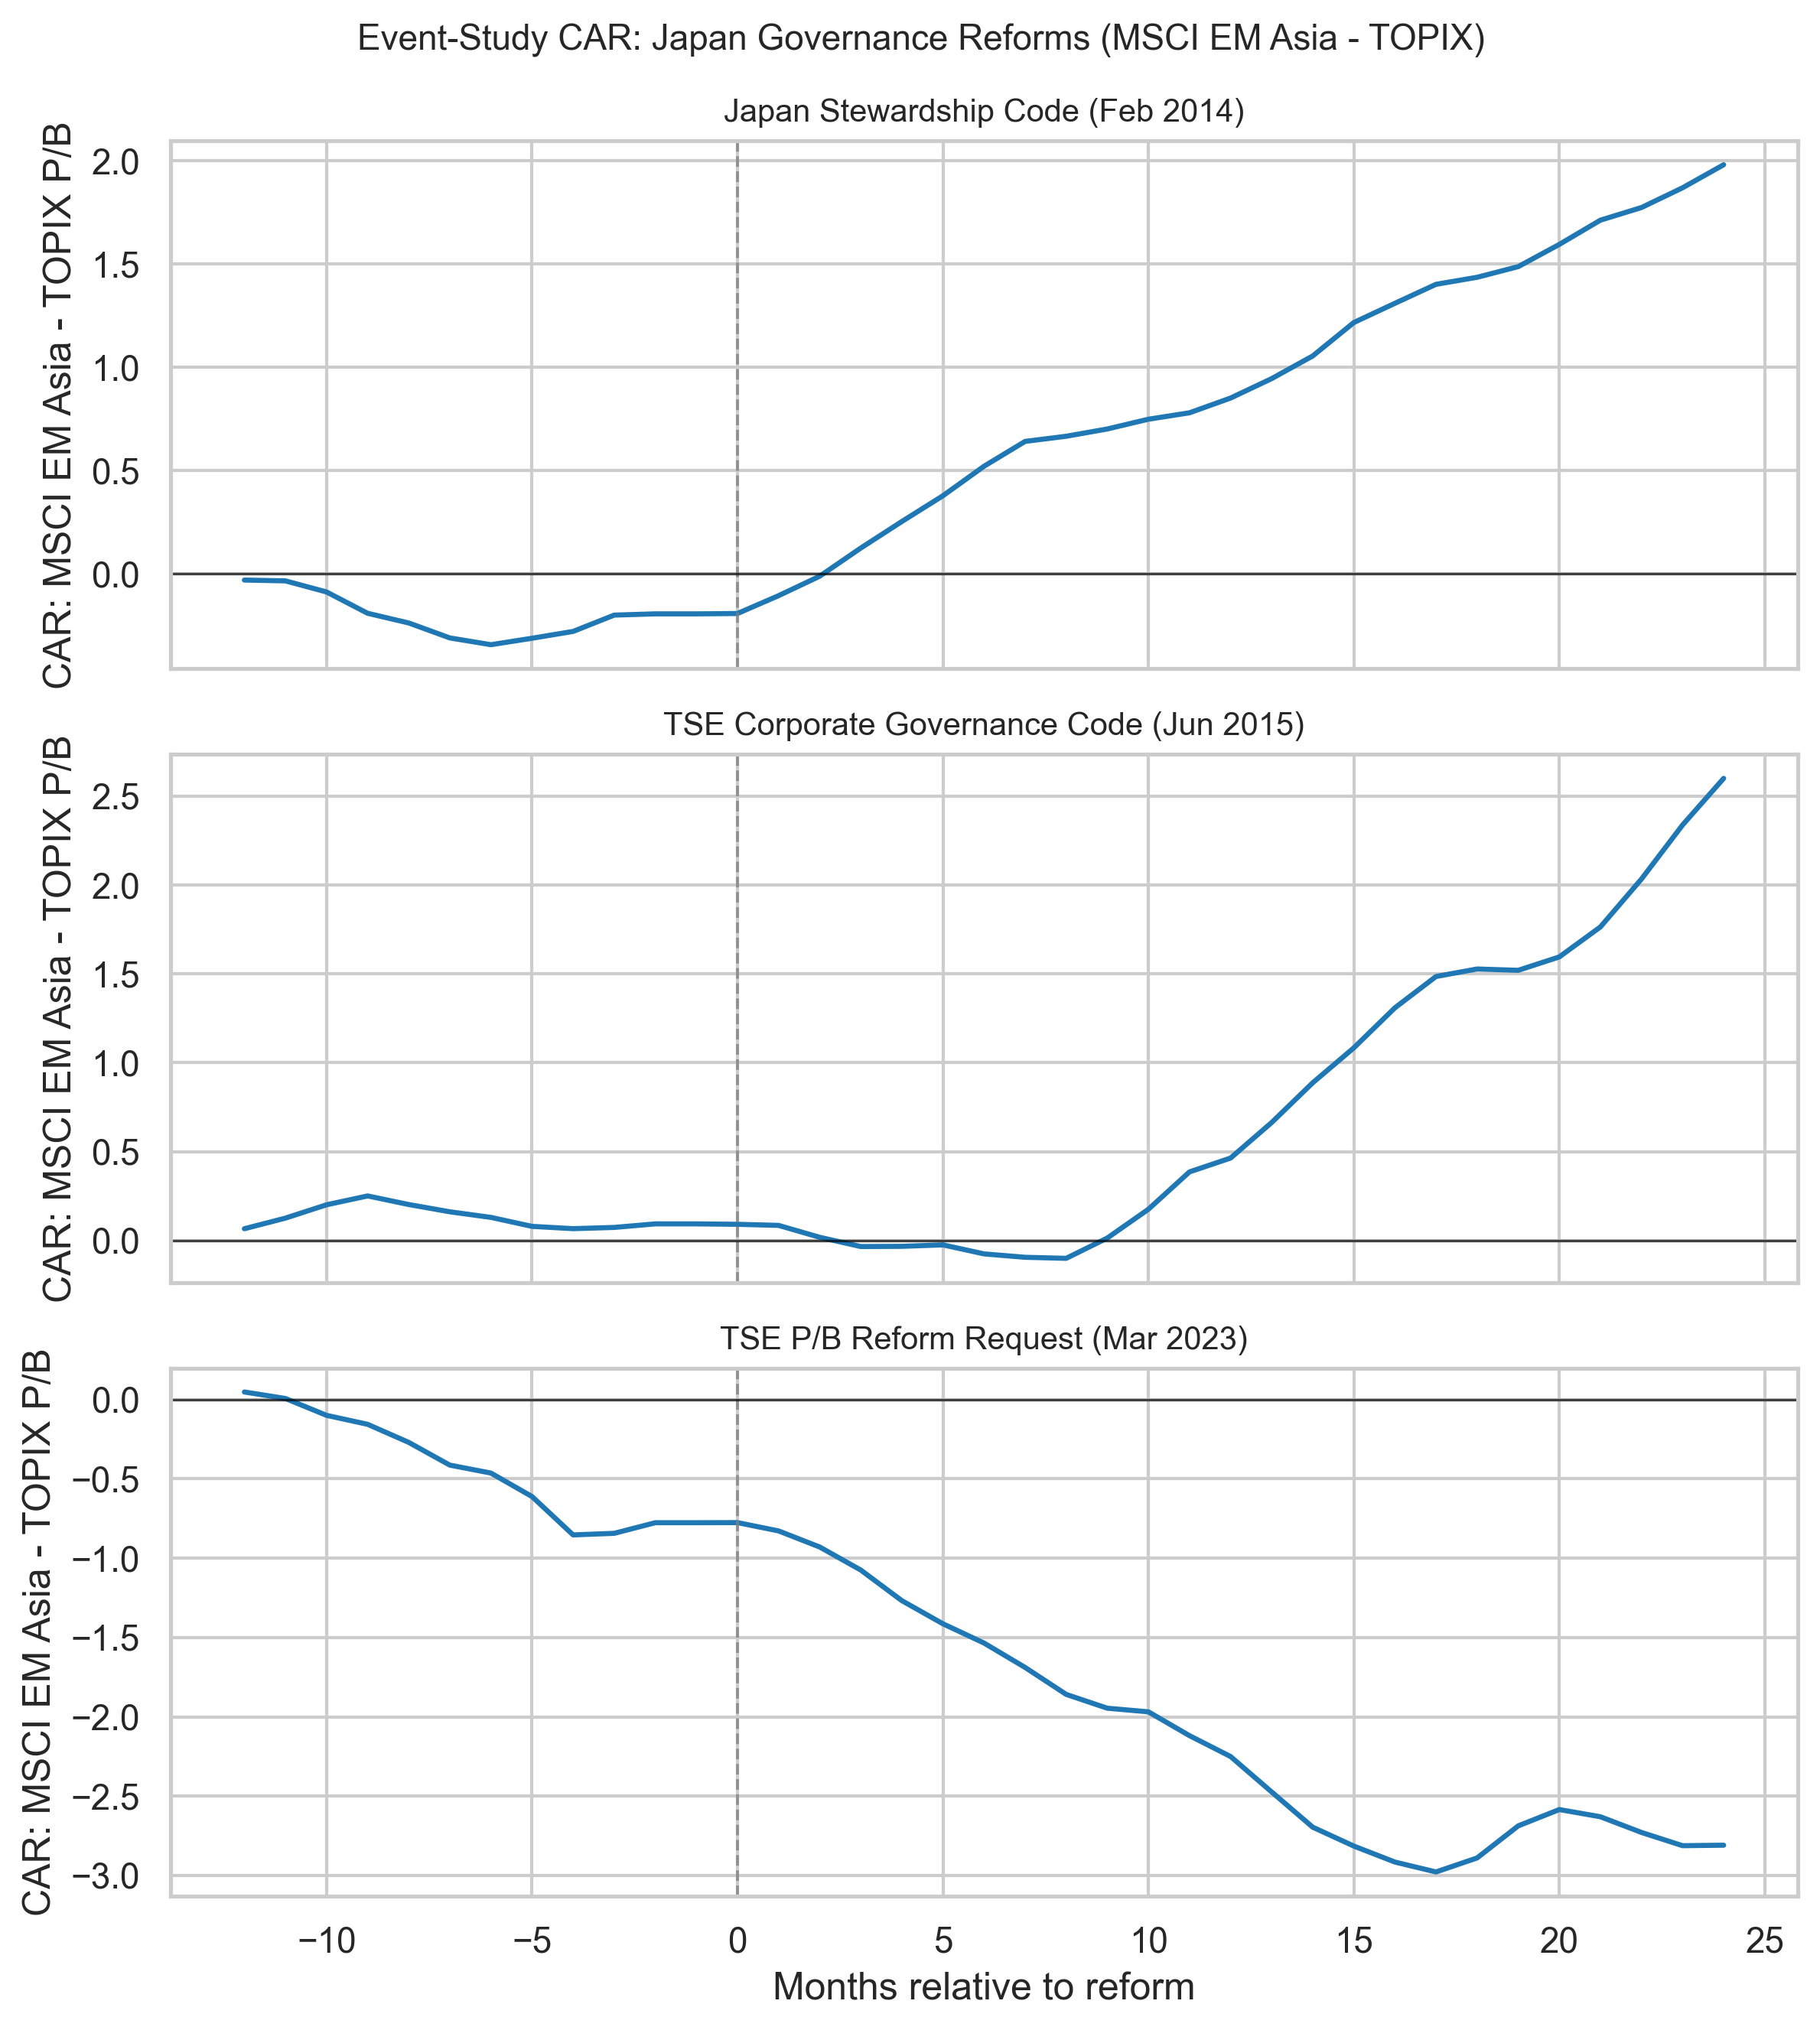
\includegraphics[width=\textwidth]{figure_asia_event_study.png}
        \caption{MSCI EM 아시아--TOPIX}
    \end{subfigure}
    \hfill
    \begin{subfigure}[b]{0.49\textwidth}
        \centering
        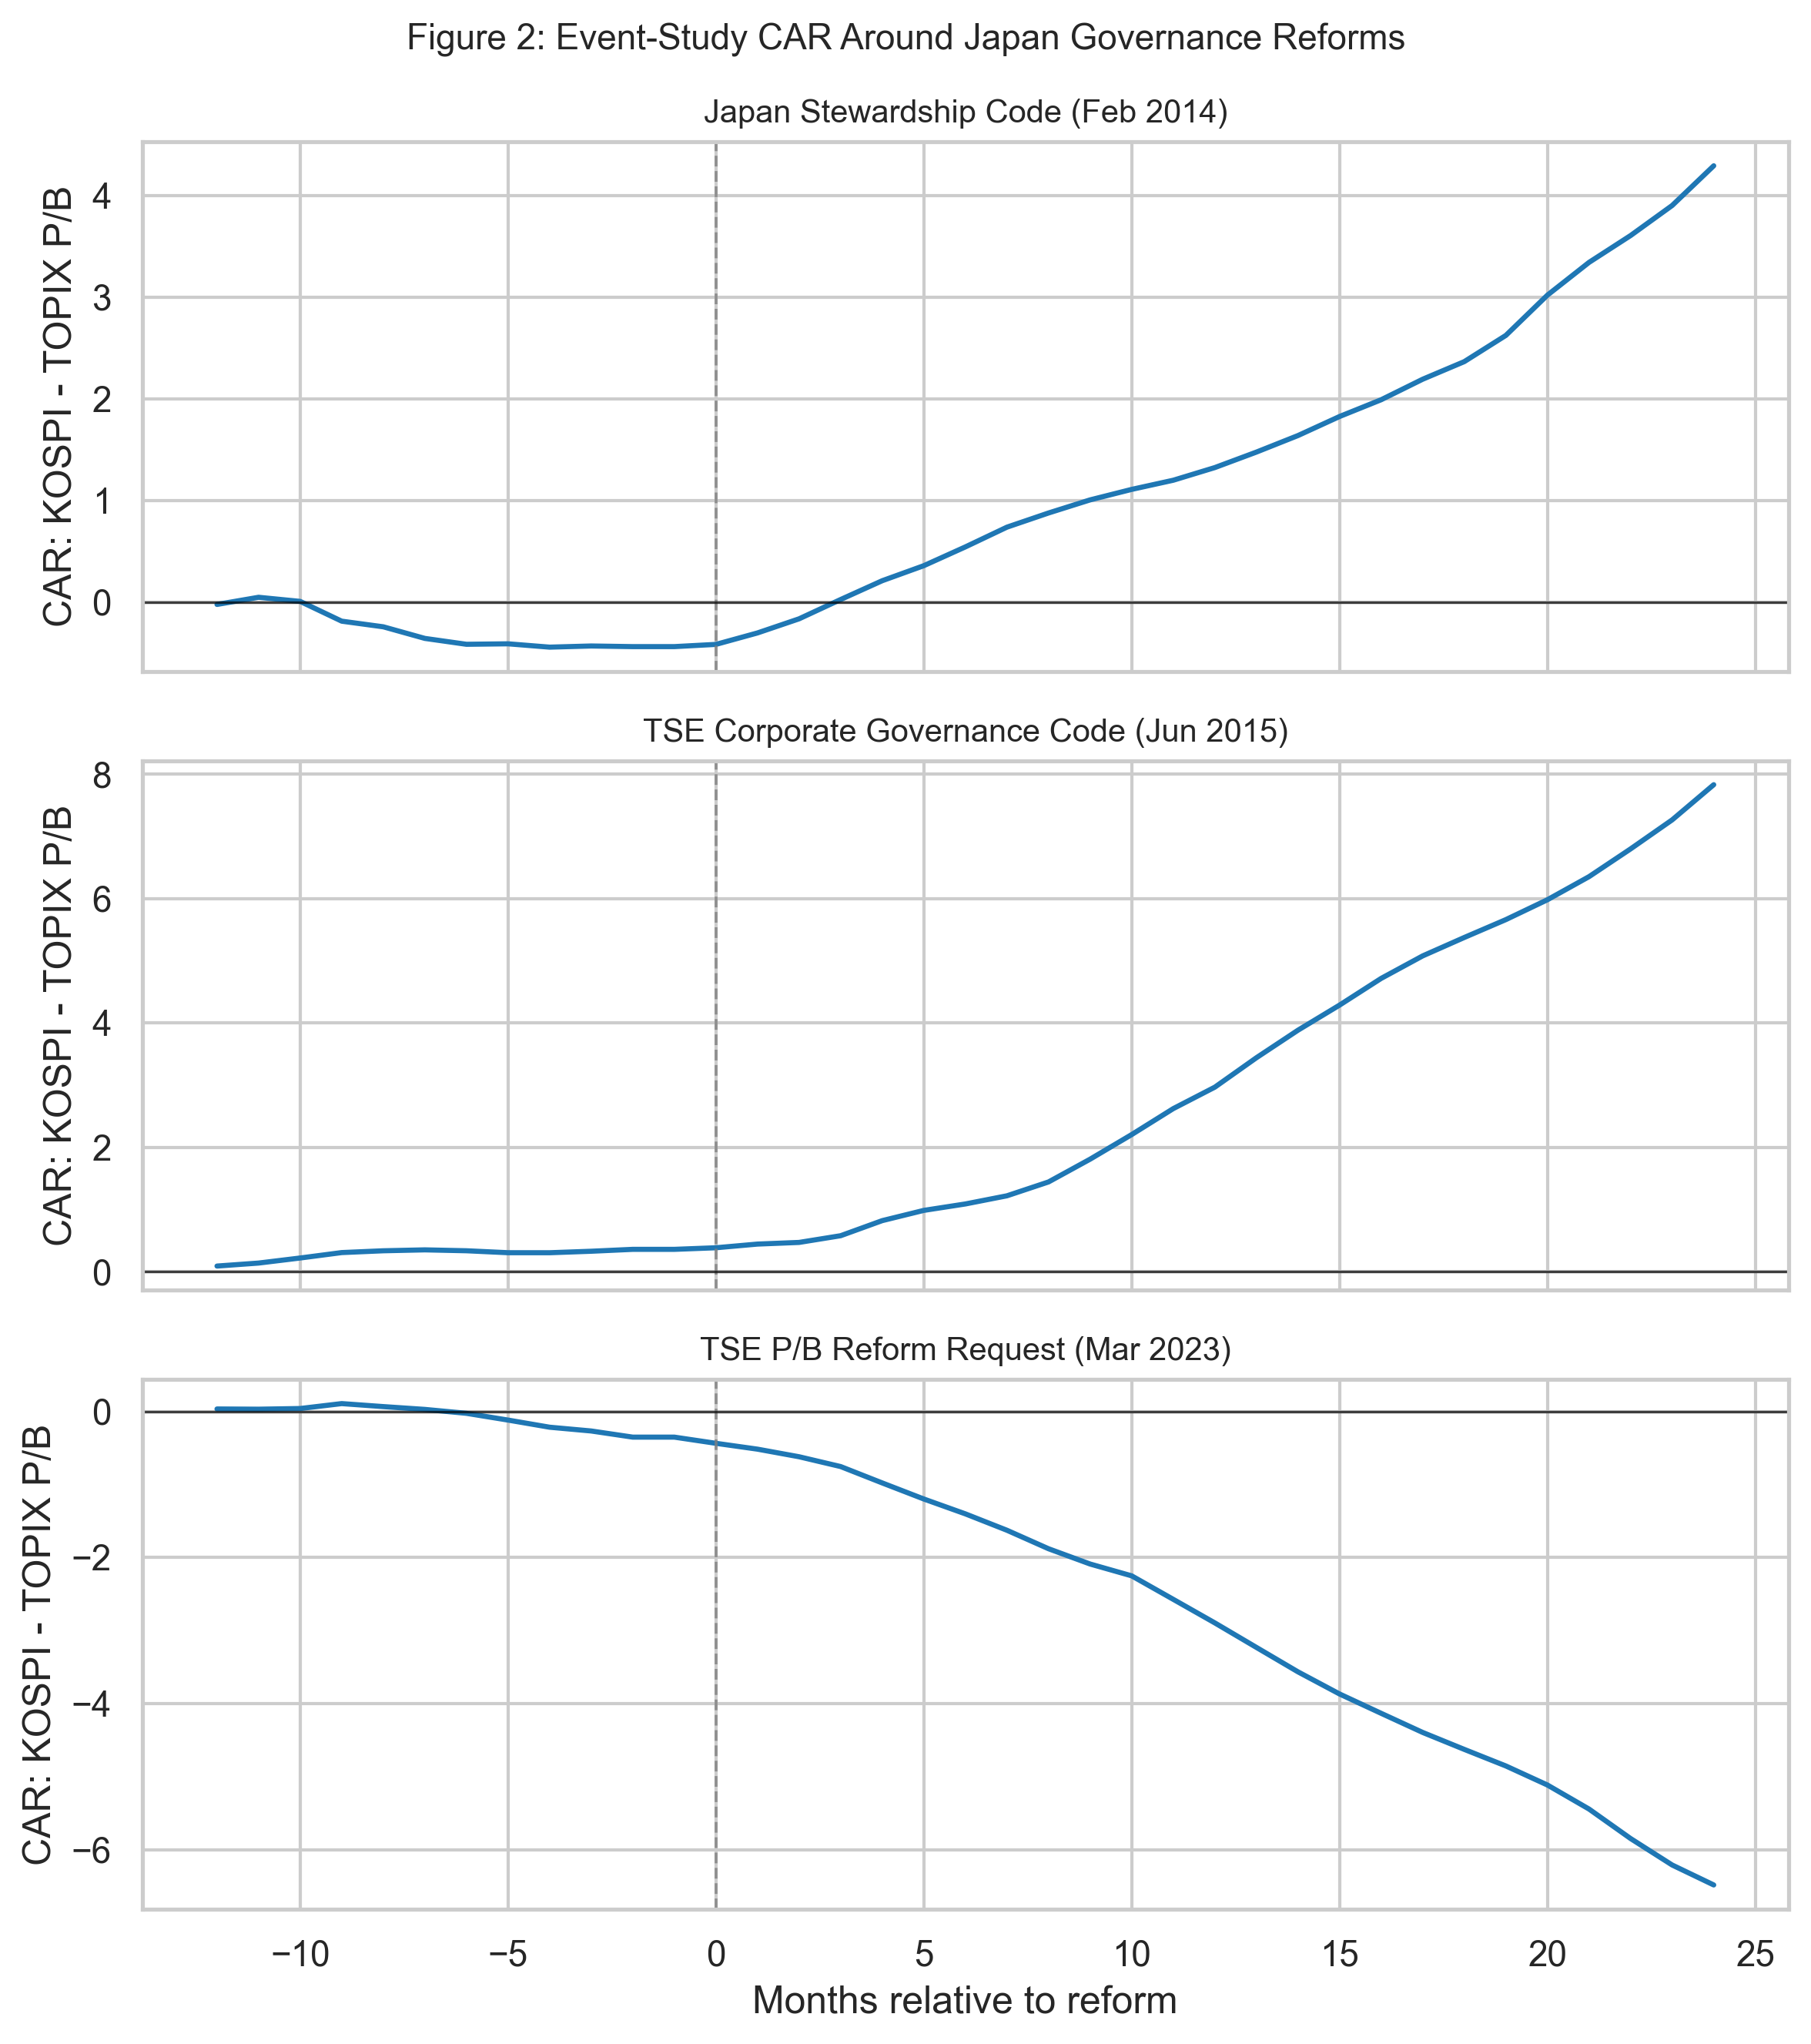
\includegraphics[width=\textwidth]{figure2_event_study.png}
        \caption{KOSPI--TOPIX}
    \end{subfigure}
    \caption{일본 지배구조 개혁 사건 연구 (event study). 2023년 TSE P/B 개혁 요청 이후 $-6.48$ P/B 포인트의 KOSPI--TOPIX 누적 스프레드가 관찰된 반면, 이전 연성 코드들 이후에는 지속적인 스프레드 변화가 나타나지 않는다.}
    \label{fig:japan_es}
\end{figure}

그림~\ref{fig:japan_followon}은 2025년 TSE 구속력 있는 의무화까지 기간을 확장한다. KOSPI--TOPIX 스프레드는 개혁 요청 시점의 $\tau=24$ 기준 $-6.48$ P/B 포인트를 넘어 추가로 확대돼, 집행 강도가 높아질수록 스프레드 이동도 커지는 패턴과 일치한다.

\begin{figure}[htbp]
    \centering
    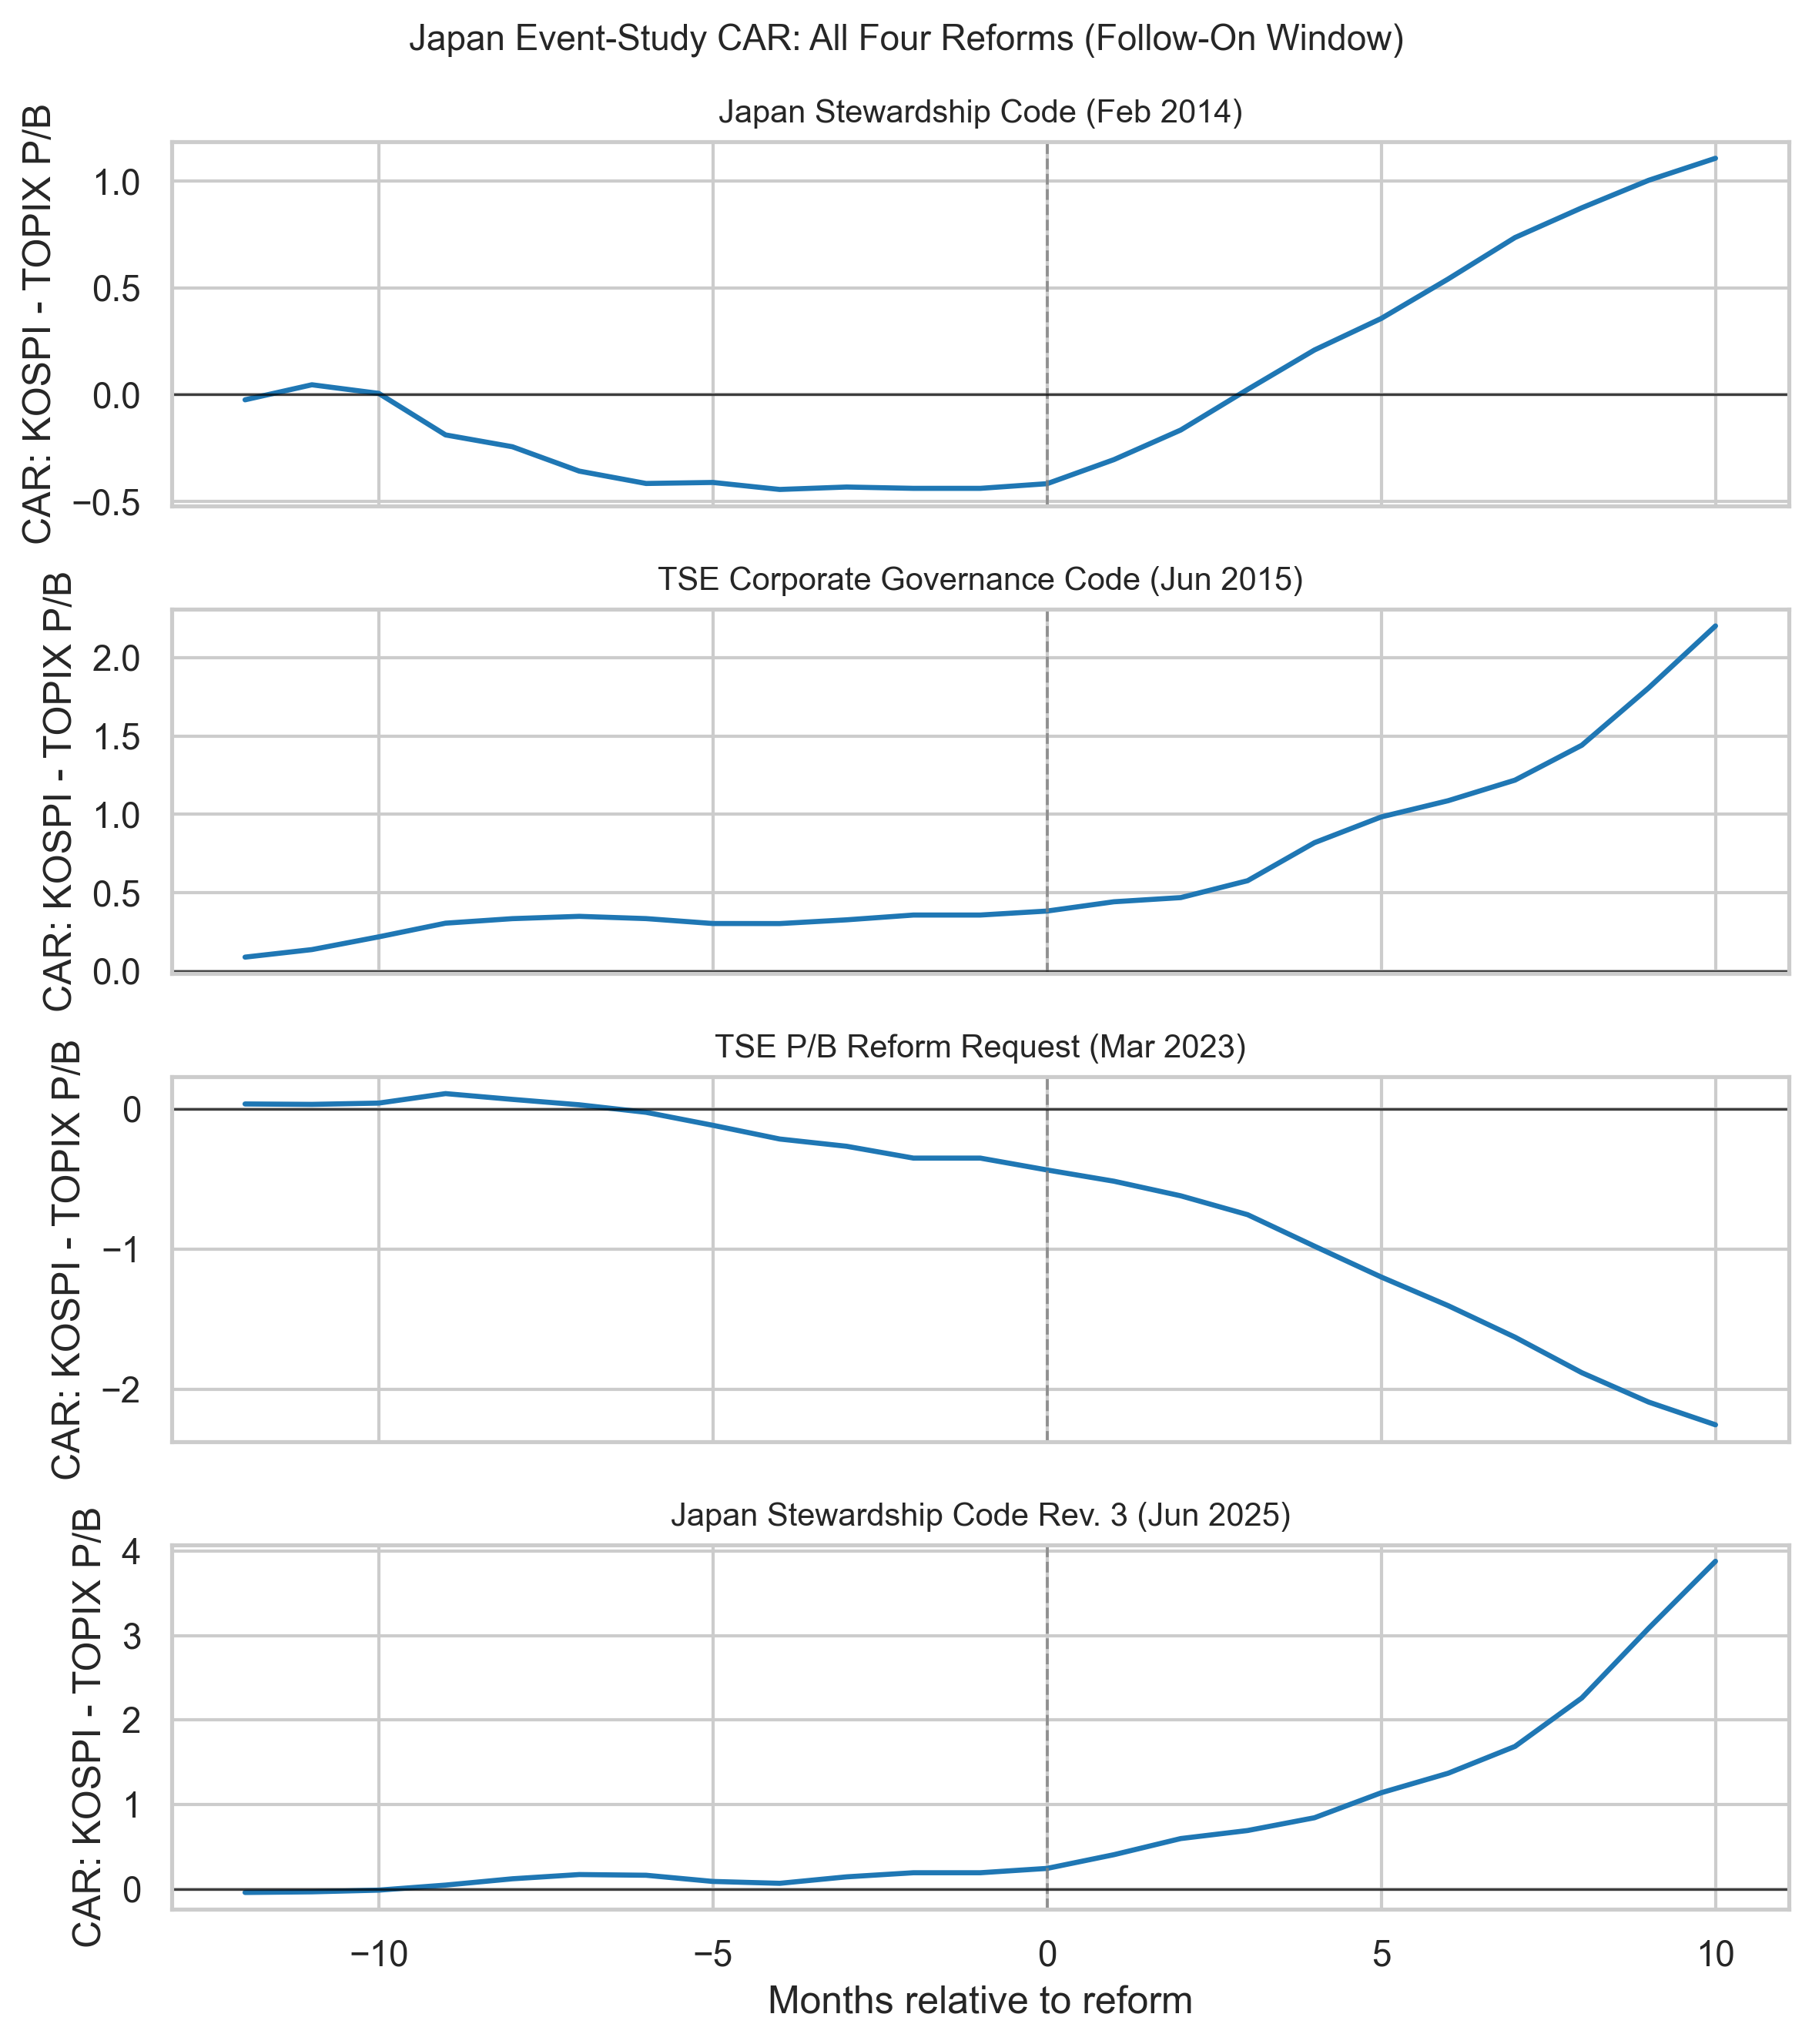
\includegraphics[width=0.95\textwidth]{figure_japan_follow_on_event_study.png}
    \caption{일본 후속 사건 연구 (event study): 2025년 TSE 구속력 있는 의무화. KOSPI--TOPIX 스프레드가 2023년 개혁 요청 시점의 $-6.48$ P/B 포인트 누적 스프레드를 넘어 추가로 확대되며, 집행 강도가 높아질수록 스프레드 이동도 커지는 패턴과 일치한다.}
    \label{fig:japan_followon}
\end{figure}

\subsection{실증 분석: 한국의 기업가치 제고 프로그램}

그림~\ref{fig:korea_es}는 한국 기업가치 제고 사건 연구 (event study)다. MSCI EM 아시아에서 KOSPI를 뺀 스프레드와 TOPIX에서 KOSPI를 뺀 스프레드 모두 세 이정표 내내 지속적으로 양(+)의 값을 기록한다---두 벤치마크 모두 KOSPI를 일관되게 상회했다는 뜻이다. 프로그램 출범(2024년 2월) 이후 MSCI EM 아시아--KOSPI CAR은 $\tau=12$에서 $+2.18$, $\tau=20$에서 $+4.14$였다. 지침 공개(2024년 5월) 이후에는 $\tau=12$에서 $+1.80$, 이행 촉진(2024년 8월) 이후에는 $\tau=12$에서 $+2.12$였다. 한국의 자율 프로그램 이후 상대적 밸류에이션에서는 아무런 개선도 나타나지 않았다.

\begin{figure}[htbp]
    \centering
    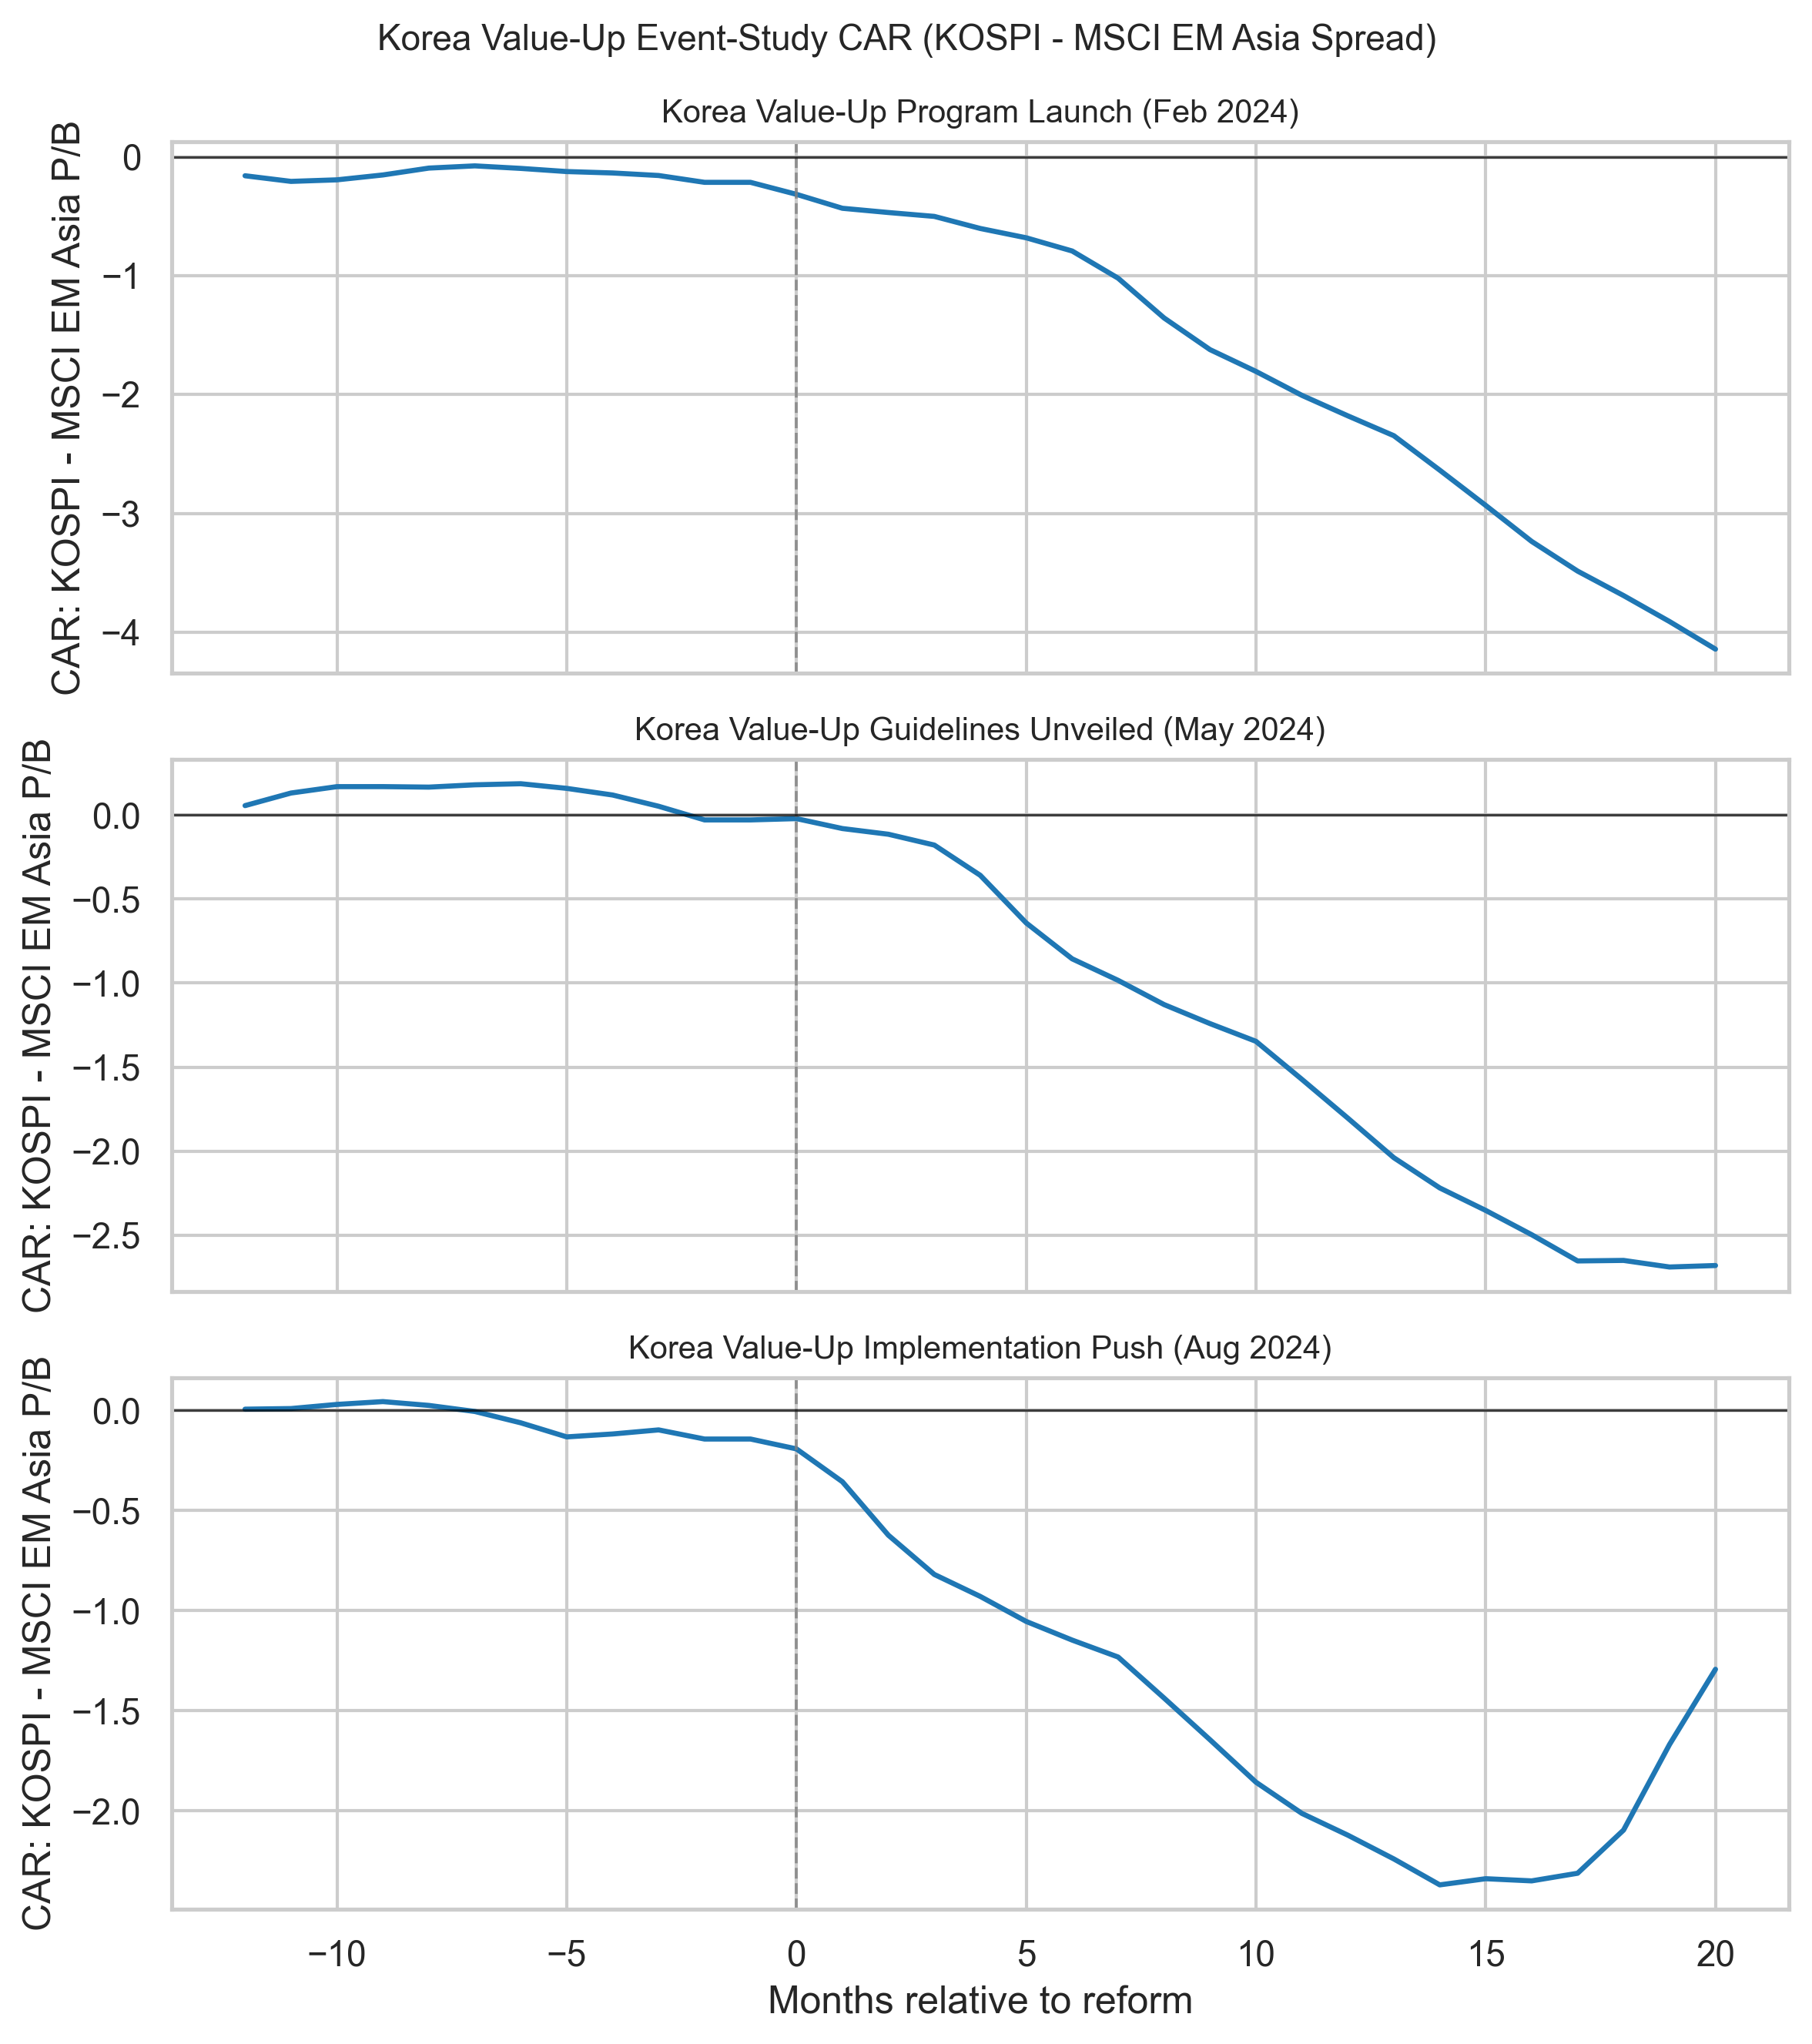
\includegraphics[width=0.95\textwidth]{figure_korea_asia_event_study.png}
    \caption{한국 기업가치 제고 사건 연구 (event study, MSCI EM 아시아--KOSPI). 세 이정표 모두 이후 MSCI EM 아시아가 KOSPI를 지속적으로 상회하는 양(+)의 누적 스프레드가 관찰된다.}
    \label{fig:korea_es}
\end{figure}

\section{지정학적 리스크 및 기타 설명}
\label{sec:geopolitical}

북한 지정학적 리스크도 코리아 디스카운트의 원인으로 자주 거론되지만, 실증 증거는 제한적이다. 예측 불가능한 핵무장 국가와 인접해 있으니 주식 리스크 프리미엄이 높아지고 밸류에이션이 낮아야 한다는 생각은 당연하다. 그러나 지정학적 리스크를 직접 통제한 다국가 연구들은 할인이 그대로 유지됨을 보여준다 \citep{kim2026korean}. 시장은 북한 위협을 고질적이고 이미 가격에 녹아든 배경 조건으로 취급할 뿐, 점진적 불확실성의 원인으로 보지 않는다는 뜻이다. 국가 간 할인 격차를 설명하는 것은 군사적 위협이 아니라 한국의 경제 정책 불확실성 지수였다 \citep{kim2025causes}.

\subsection{지정학적 리스크 반증 (Falsification)}

검증을 공식화하기 위해, TOPIX P/B와 연도 고정 효과 (year fixed effects)를 통제하면서 KOSPI P/B를 한국 GPR 고조 더미 (dummy, GPRC\_KOR, \citealt{caldara2022}, 75번째 백분위수 초과)에 회귀했다. 관측치는 2004년 1월부터 2024년 12월까지 252개월이다. GPR 계수는 $-0.016$ ($t=-0.84$, $p=0.40$)---통계적으로 0과 구분되지 않고, 평균 KOSPI--TOPIX 스프레드의 10분의 1 미만으로 경제적으로도 무시할 수준이다. 이 설정 (specification)은 GPRC\_KOR이 비지정학적 이유로 한국 밸류에이션을 낮추는 글로벌 리스크 오프 에피소드도 포착할 수 있어, 오히려 효과를 발견하는 방향으로 편향돼 있다. 그런데도 아무것도 발견되지 않았다. 그림~\ref{fig:geo_risk}는 GPR 고조 에피소드와 함께 KOSPI P/B 계열을 보여주는데, 가장 심각한 위기 국면에서도 체계적인 공동 움직임이 나타나지 않는다. 이 귀무 결과는 지정학적 \emph{충격}의 가격 형성에 관한 것이며, 표본 전반에 걸쳐 일정하여 절편에 흡수되는 구조적 수준 프리미엄의 가능성까지 배제하지는 않는다.

\begin{figure}[htbp]
    \centering
    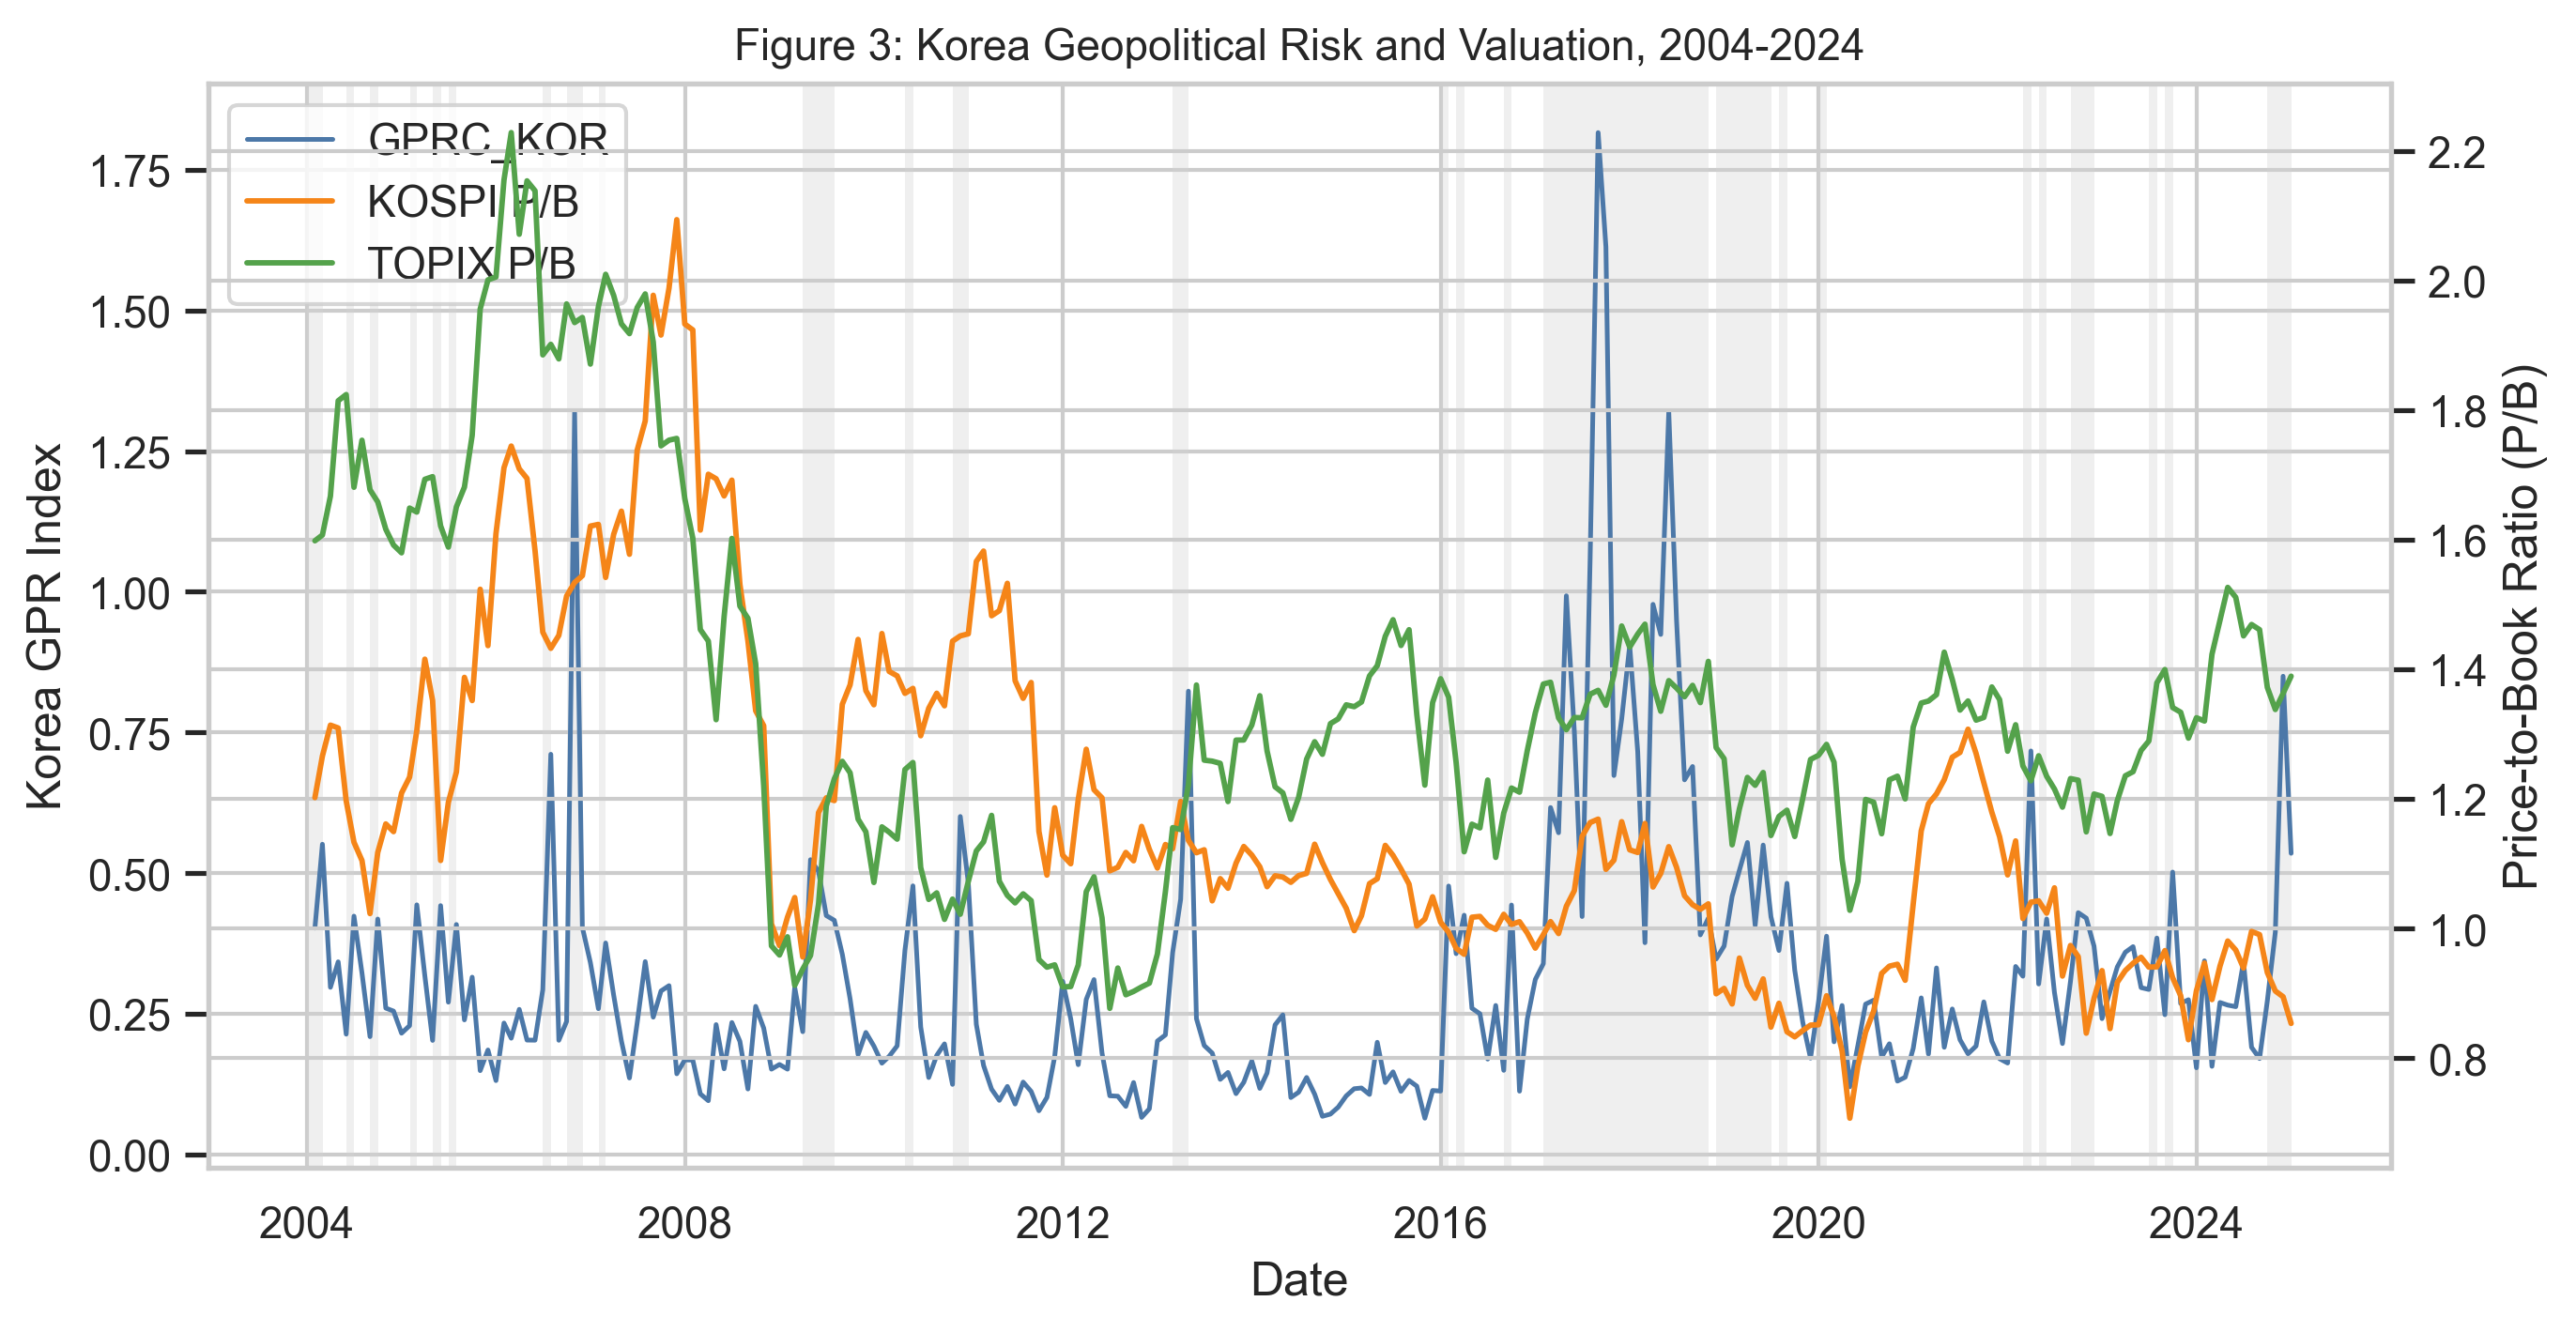
\includegraphics[width=0.95\textwidth]{figure3_geo_risk.png}
    \caption{KOSPI P/B와 북한 지정학적 리스크 고조 에피소드. 음영 영역은 한국 GPR 지수(GPRC\_KOR)가 75번째 백분위수를 초과한 기간이다. 체계적인 공동 움직임은 나타나지 않으며, 회귀 계수는 $-0.016$ ($t=-0.84$, $p=0.40$)이다.}
    \label{fig:geo_risk}
\end{figure}

\section{종합 및 정책적 함의}
\label{sec:synthesis}

코리아 디스카운트 완화에는 자율 지침이 아닌 집행 신뢰성을 갖춘 개혁이 필요하다.

이 보고서의 핵심 실증 패턴은 일본 지배구조 개혁의 단계적 에스컬레이션이다. 2014년·2015년 자율 코드 이후 지속적인 TOPIX 재평가는 나타나지 않았다. 형식상 여전히 자율이었지만 월별 공개 준수 현황표와 암묵적 재분류 압박으로 뒷받침된 2023년 TSE P/B 개혁 요청 이후 24개월 동안 KOSPI--TOPIX 누적 스프레드는 $-6.48$ P/B 포인트에 달했다. 자동 강등을 수반한 2025년 구속력 있는 의무화 이후 스프레드는 추가로 확대됐다 (그림~\ref{fig:japan_followon}). 집행 강도가 단계적으로 높아질수록 데이터상의 스프레드 이동도 커진 것이다. 한국의 2024년 자율적 기업가치 제고 프로그램에서는 세 이정표 모두에서 MSCI EM 아시아가 KOSPI를 지속적으로 상회했고, 양(+)의 누적 스프레드가 이어졌다 (그림~\ref{fig:korea_es}).

NPS를 통한 기관투자자 스튜어드십은 조건부 개선을 이끌어냈지만 \citep{kim2022nps_esg, lee2026esg}, 시장은 NPS의 반대 투표 공표에 반응하지 않았고 \citep{kim2014nps} 스튜어드십 코드 채택도 다변량 검정에서 통계적 유의성에 이르지 못했다 \citep{park2021stewardship}. 이는 구조적 개혁 없이 자율적 관여만으로는 집행 신뢰성을 확보하기 어렵다는 더 넓은 패턴과 일치한다. 외국인 투자자 규율은 보완적 채널을 제공하지만 \citep{joo2026foreign, kim2015foreign}, 그 효과는 외국인 소유권을 높이는 시장 접근성 개혁이 수반될 때에만 발현된다. 지정학적 리스크 설명도 신뢰성이 낮다: 한국 GPR 계수는 $-0.016$ ($t=-0.84$, $p=0.40$)으로 경제적으로 무시할 수준이며 통계적으로도 0과 구분되지 않는다.

이사의 수탁 의무를 주주로 확대한 한국의 2025년 상법 개정은 할인 기업들에 유의미하게 긍정적인 비정상 수익률을 발생시켜 \citep{kang2026commercial} 강성 규범 메커니즘을 검증하고 실질적인 변화를 이뤄냈다. 그러나 수탁 의무 확대는 소송을 통해 작동하는 반면, 일본의 TSE 의무화는 거래소 차원에서 작동한다. 현재 스프레드를 해석할 때는 두 가지 교란 요인도 봐야 한다. 첫째, 반도체 호황은 한국(SK하이닉스, 삼성전자)과 대만(TSMC) 주식시장 모두에 이례적인 상승을 가져다줬다. 이는 지배구조 개혁과 무관한 경기 순환적 요인으로, KOSPI와 동종 시장의 격차를 압축시켰다. 이 점을 감안하면 단기적 한국 재평가를 액면 그대로 해석하기는 어렵다. CAR를 떠나서 TOPIX도 2025--2026년 사상 최고치를 기록했다---1989년 버블 정점 이후 처음으로 그 수준을 돌파하며 일본의 "잃어버린 수십 년"에 마침표를 찍었다. 이 보고서에서 분석한 개혁 시퀀스가 TOPIX의 역사적 회복과 궤를 같이한다는 것은 사건 연구의 기술적 패턴과 일치하지만, 동시에 인과적 해석의 어려움도 보여준다: TOPIX의 역사적 상승은 지배구조 개혁, 엔화 약세, 외국인 자금 유입, 내수 회복이 복합적으로 작용한 결과로, 기술적 스프레드 추정치만으로는 이를 분리할 수 없다. 한국의 2025년 상법이 이에 버금가는 재평가를 이끌어낼 수 있는지는 반도체 경기 사이클이 성숙해지면서 더 명확해질 것이다.

{\singlespacing
\bibliographystyle{plainnat}
\bibliography{references}
}

\begin{center}
    "I pledge my honor that I have not violated the honor code during this assignment."\\
    \vspace{0.5cm}
    \textbf{Daniel Jung}
\end{center}

\end{document}
